\section{Algorithmen}
\label{sec:algorithmen}

Zur Auswertung der gesammelten Messaden werden wie in Abbildung
\ref{fig:algo} gezeigt, bestimmte Algorithmen benötigt, um die
Position zu bestimmen. Zwei Grundlegende Methoden zur Bestimmung der
Position sind \textbf{Triangulation} und \textbf{Trilateration}, die
die Grundlage zu anderen Verfahren bilden.

\subsection{Triangulation}

Wird das \ac{AoA} Verfahren verwendet müssen mindestens zwei ortsfeste
Koten $A$ und $B$ so wie die Einfalswinkel $\alpha$ und $\beta$ der
Signale bekannt sein. Dann kann mittels Triangulation (Abbildung
\ref{fig:triang}) die Position eines weiteren Knoten $C$ berechnet
werden. Der Knoten $C$ kann wiederum ein stationärer oder ein mobieler
Knoten sein.

\begin{figure}[h!]
  \centering
  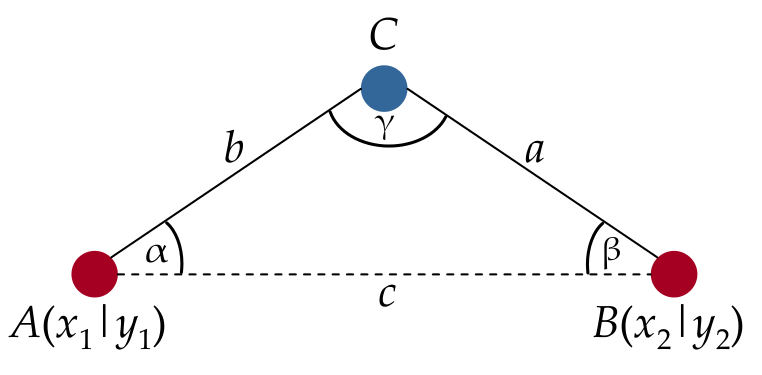
\includegraphics[scale=0.3]{img/triang}

  \caption{Triangulation}
  \label{fig:triang}
\end{figure}

Der Grundgedanke dabei ist, dass theoretisch mit nur zwei bekannten,
ortsfesten Knoten, die Position aller Nachbarn berechnet werden kann.
Sind dabei alle Knoten stationär, ist dies auch möglich, bei mobielen
Knoten kann dies allerdings Problematisch werden, da die Position des
Knotens sich permanent verändern kann. Zudem ist die Genauigkeit der
Triangulation bei mobilen Sensoren sehr schlecht und die Position kann
durch den hohen Messfehler nicht exakt bestimmt werden.
\cite{roehrig2009} 

Die Berechnung mittels Triangulation ist für einen \ac{uC} nicht sehr
aufwendig, da sie nur den Sinus- oder Cosinussatz verwendet. (Gleichung
\ref{eq:triang})

\pagebreak
\begin{framed}
\begin{equation}
  \label{eq:triang}
  c = \sqrt{(B_{x)} - A_{x})^2 + (B_{y} - A_{y})^2}
  ~~~~~~~~
  \varphi = arctan(\frac{B_{y} - A_{y}}{B_{x}} - A_{x})
\end{equation}
\begin{equation*}
  b = c \cdot \frac{sin(\beta)}{sin(\alpha + \beta)}
\end{equation*}
~\\
\begin{equation*}
  C_{x} = A_{x} + b \cdot cos(\varphi)
  ~~~~~~~~
  C_{y} = A_{x} + b \cdot sin(\varphi)
\end{equation*}
\end{framed}
\myequations{Triangulation}


\subsection{Trilateration}

Werden Verfahren wie \ac{ToA}, \ac{TDoA} oder \ac{RToF} eingesetzt,
sind die Winkel der Signale nicht bekannt. Hier werden mindestens
drei ortsfeste Knoten benötigt, um die Position zu einem weiteren
Knoten zu berechnen. Ein weiterer Vorteil der Trilateration ist, dass
die Hardware Anforderungen zur Messung des Einfallwinkels wesentlich
höher sind, als eine reine Distanzmessung. \cite{roehrig2009} 

\begin{figure}[h!]
  \centering
  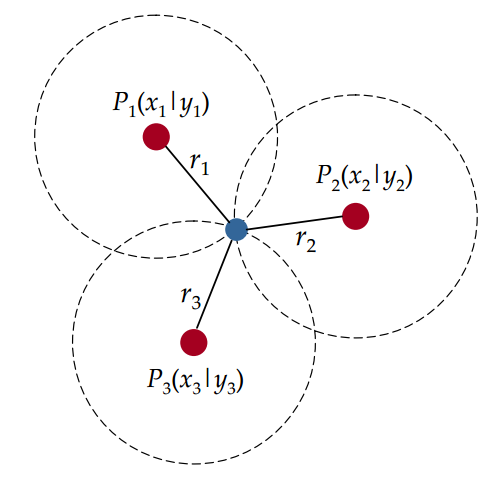
\includegraphics[scale=0.5]{img/trilat}

  \caption{Trilateration}
  \label{fig:trilat}
\end{figure}

Für die Distanz zu den Knoten $P_{¹}$, $P_{2}$ und $P_{3}$ gilt:

\begin{framed}
\begin{equation}
  \label{eq:trilat1}
  r_{i} = \sqrt{(p_{x} - x_{i})^{²} + (p_{y} - y_{i})^{2}}
\end{equation}
\end{framed}
\myequations{Trilateration: Distanz zu stationären Knoten}

Die Position des vierten Knoten lässt sich dann über das
Gleichungssystem \ref{eq:trilat2} berechnen.

\begin{framed}
\begin{equation}
  \label{eq:trilat2}
  \begin{pmatrix}
    P_{x} \\
    P_{y}
  \end{pmatrix}
  =
  H^{-1} \cdot z
\end{equation}
\begin{equation*}
  H = 
  \begin{bmatrix}
    2 \cdot x_{1} - 2 \cdot x_{2} & 2 \cdot y_{1} - 2 \cdot y_{2} \\
    2 \cdot x_{1} - 2 \cdot x_{3} & 2 \cdot y_{1} - 2 \cdot y_{3}
  \end{bmatrix}
\end{equation*}
\begin{equation*}
  z = 
  \begin{pmatrix}
    r_{2}^2 - r_{1}^2 + x_{1}^2 - x_{2}^2 + y_{1}^2 - y_{2}^2 \\
    r_{3}^2 - r_{1}^2 + x_{1}^2 - x_{3}^2 + y_{1}^2 - y_{3}^2
  \end{pmatrix}
\end{equation*}
\end{framed}
\myequations{Trilateration: Gleichungssystem}


\subsection{Weiterführende Algorithmen}

Wie bereits beschrieben, bieten die beiden geziegten Verfahren nur
ungenaue Ergebnisse, vor allem bei mobielen Knoten ist der Fehler sehr
groß. Auß diesem Grund werden weitere Verfahren benötigt, um die
Wahrscheinlichkeit zu maximieren, dass die berechnete Position stimmt.

% TODO Algos hinzufügen 